\documentclass{article}

% Packages
\usepackage{amsmath}    
\usepackage{amsfonts}  
\usepackage{amssymb}    
\usepackage{graphicx}   
\usepackage{hyperref}   
\usepackage{booktabs}  
\usepackage{geometry}   
\usepackage{natbib}     
\usepackage{authblk}    
\usepackage{subcaption}
\usepackage{xcolor}
\usepackage{siunitx}


\geometry{left=25mm, right=25mm, top=25mm, bottom=25mm}
\newcommand{\reddashedline}{\textcolor{red}{---}}
\title{Planetary Mission}

\begin{document}
	
	
\section{Introduction}
The  PoliMi  Space  Agency  wants  to  launch  a  Planetary  Explorer  Mission,  to  perform  Earth Observation. This section carries out relevant orbital analysis and groundtrack estimation while also considering two perturbation models. A modified groundtrack was proposed for a repeating groundtrack, and two propagation methods are used to perform the analysis which are then compared. A comparison between the real data of a satellite and its analytical results obtained with the code model is also performed for model validity. 

\subsection{Nominal Orbit}

From the provided orbital parameters this satellite heavily contains geosynchronous orbital characteristics. Hence, the altitude at perigee is chosen as 35786 km - where it is possible to see the moon and J2 perturbation effect. $\Omega, \omega, \text{ and } f_0$ are chosen arbitrarily.

%citation for GSO: https://www.esa.int/ESA_Multimedia/Images/2020/03/Geostationary_orbit

\begin{table}[ht]
	\centering
	\label{tab:keplerian_elements}
	\begin{tabular}{|c|c|c|c|c|c|}
		\hline
		a [km] & e [-] & i [°] & $\Omega$ [°] & $\omega$ [°] & altitude at perigee [km] \\
		\hline
		42159 & 0.0007 & 32.5934 & 0 & 85 & 35786 \\
		\hline
	\end{tabular}
	\caption{Keplerian elements of the orbit.}
	\label{tab:keplerian_elements}
\end{table}
\begin{flushleft}
	The unperturbed nominal orbit is propagated as below in the Earth-centered reference frame:
\end{flushleft}

\begin{figure}[ht]
	\centering
	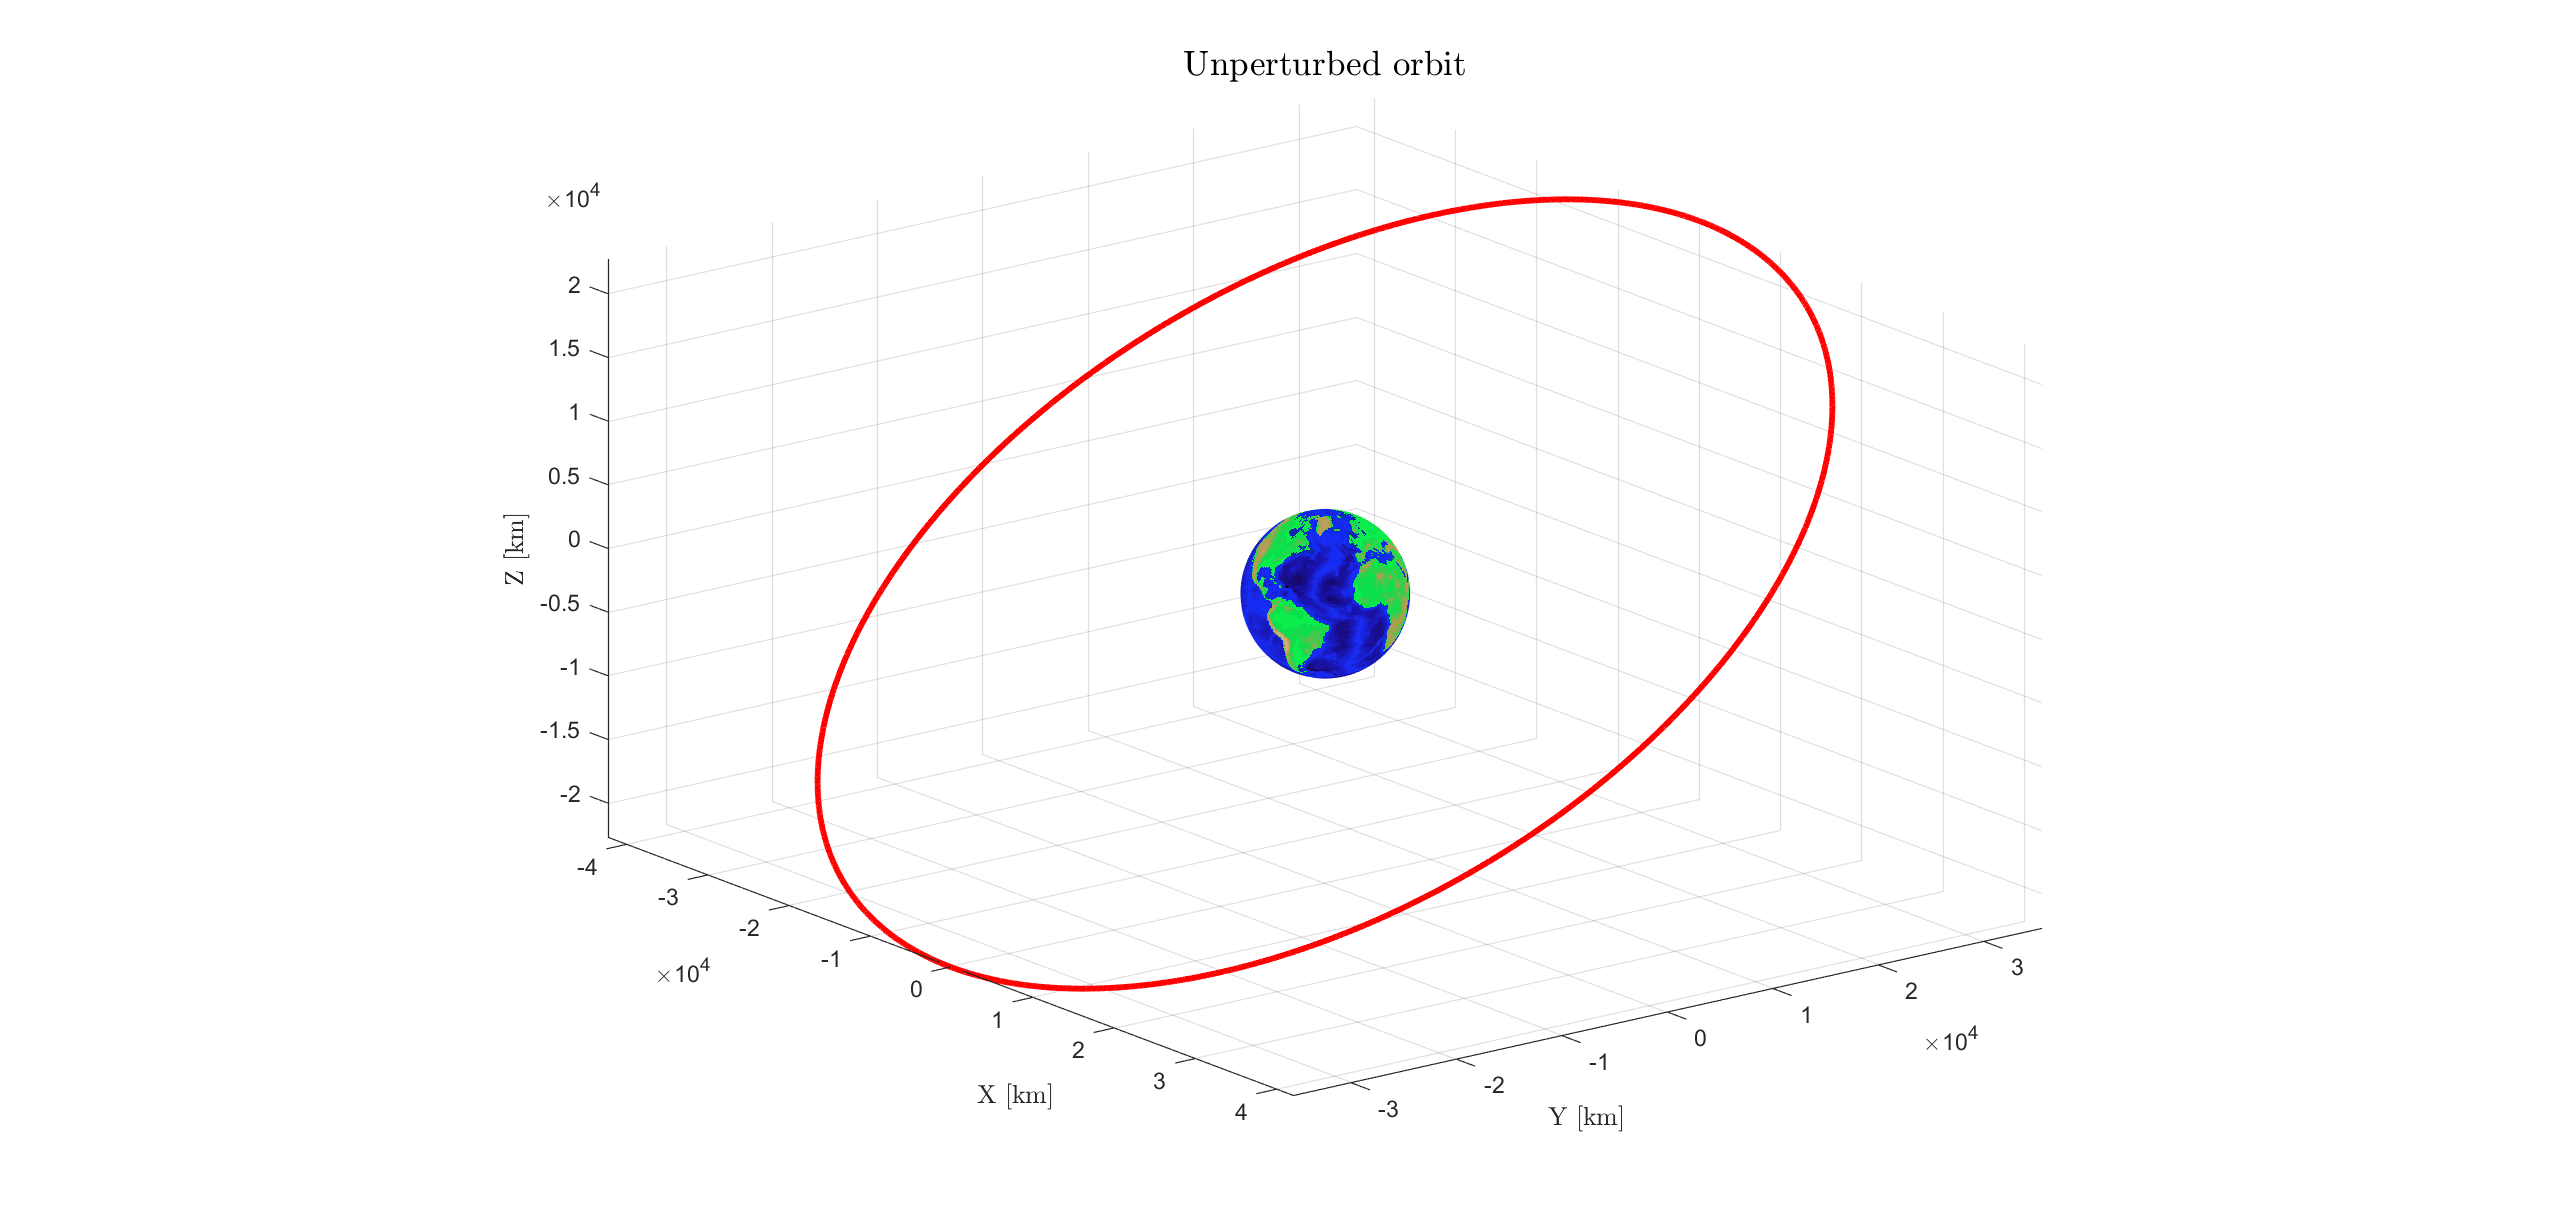
\includegraphics[width=0.8\textwidth]{nominal_orbit.png}
	\caption{Assigned orbit.}
	\label{fig:nominal_orbit}
\end{figure}

\section{Groundtrack}
The satellite's orbit is propagated to compute its groundtrack. The motion of the spacecraft is assumed to be a perturbed two body problem in Cartesian coordinates, described by the equation:
\[
\dot{\mathbf{r}} = -\frac{\mu}{r^3} \mathbf{r} + \mathbf{a}_{\text{perturbation}}
\]
This is solved using Matlab's \texttt{ode113} function, with a relative tolerance of \(1 \times 10^{-12}\) and absolute tolerance of \(1 \times 10^{-12}\).

%citation for formula: Curtis

\subsection{Unperturbed Groundtrack}
\subsubsection{Nominal Orbit Groundtrack}

The first required analysis of the ground track is for the nominal orbit considering an unperturbed case, where the $\mathbf{a}_{perturbation}$ in equation is null. The ground track was propagated for a period of 1 orbit of the satellite, 1 day and 10 days, as shown below.\\
\begin{figure}[ht]
	\centering
	% First row with two figures
	\begin{subfigure}[b]{0.45\textwidth}
		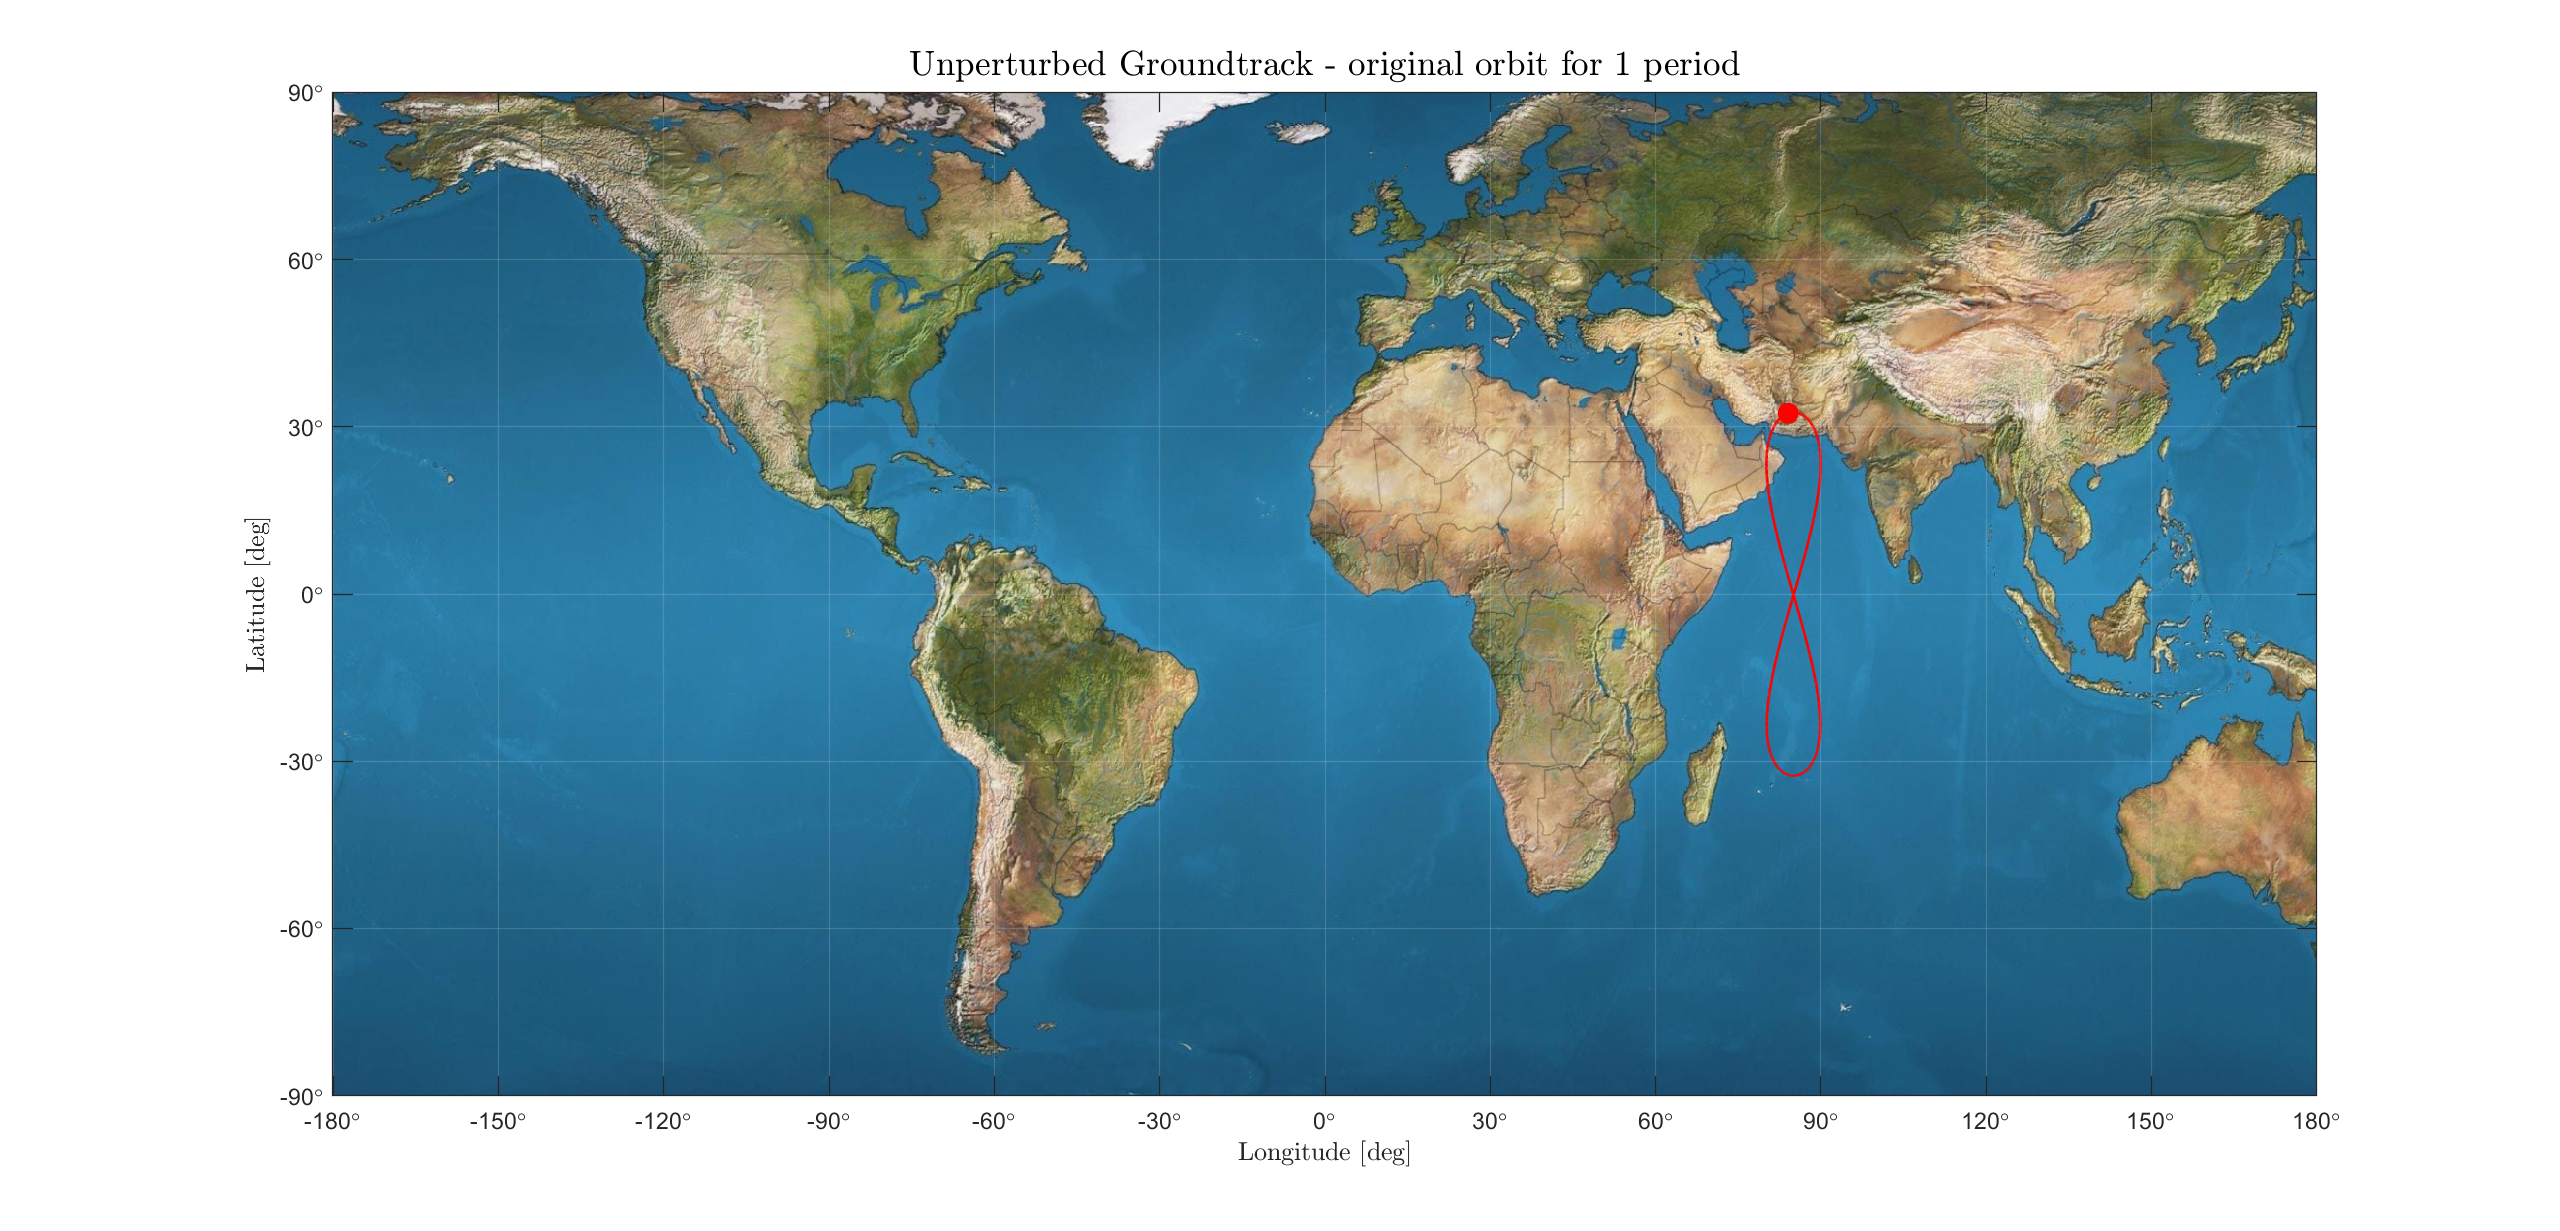
\includegraphics[width=\textwidth]{ug1orb.png}
		\caption{}
		\label{fig:1a}
	\end{subfigure}
	\hfill
	\begin{subfigure}[b]{0.45\textwidth}
		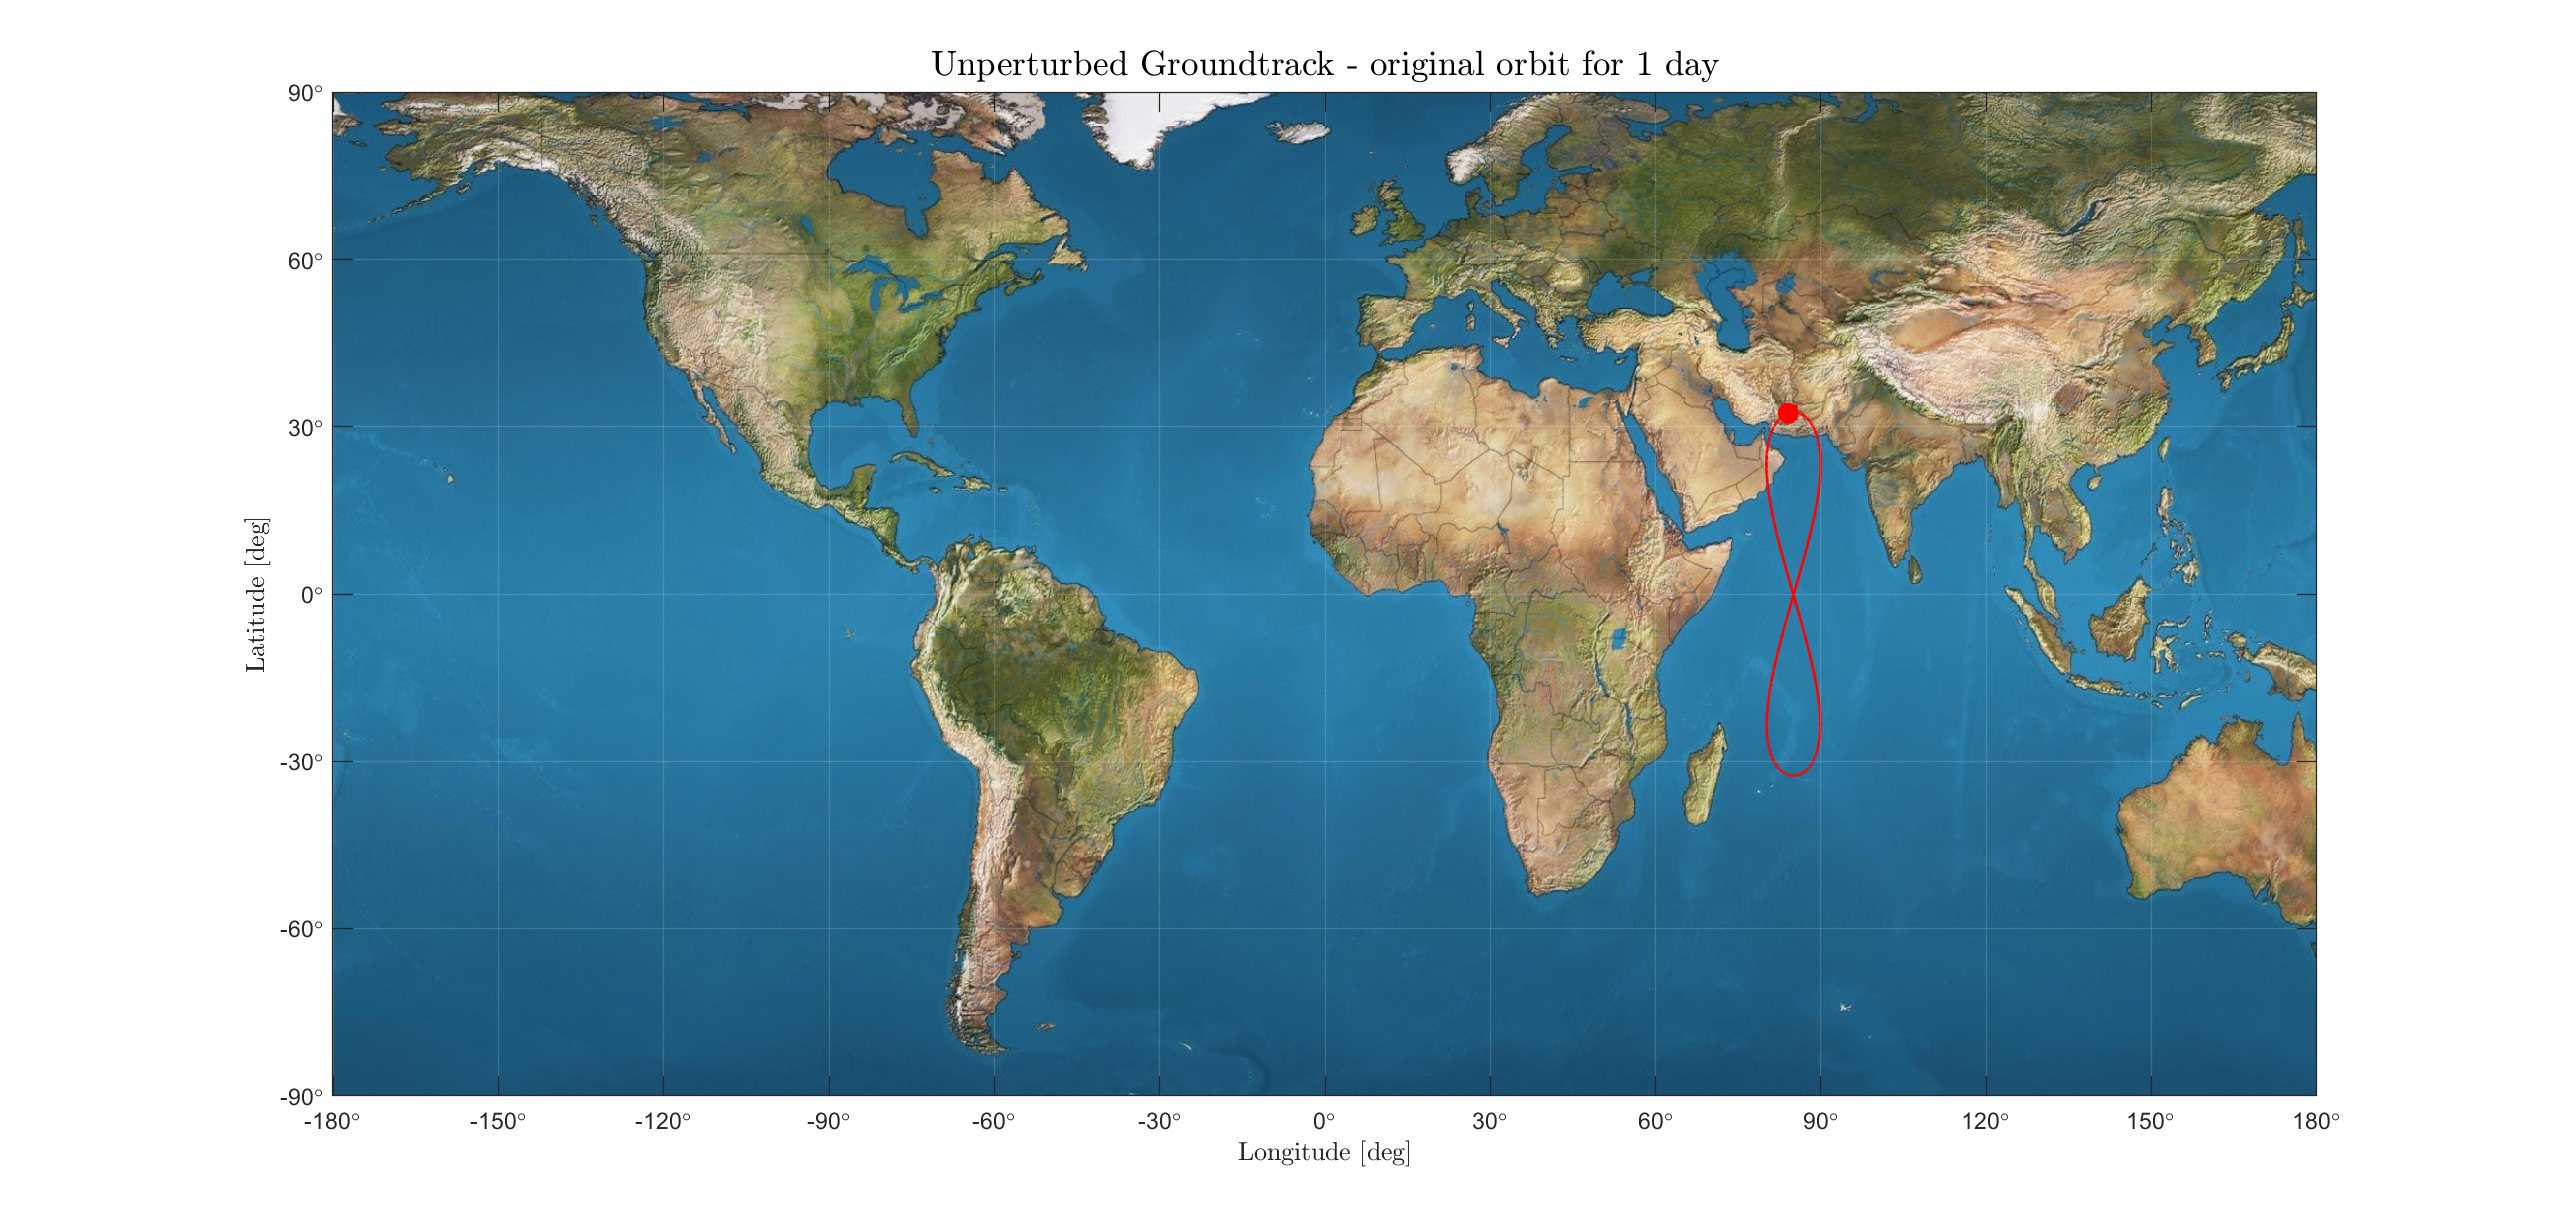
\includegraphics[width=\textwidth]{ug1d.png}
		\caption{}
		\label{fig:1b}
	\end{subfigure}
	
	% Second row with two figures
	\vspace{1cm} % Adjust the vertical spacing as needed
	\begin{subfigure}[b]{0.45\textwidth}
		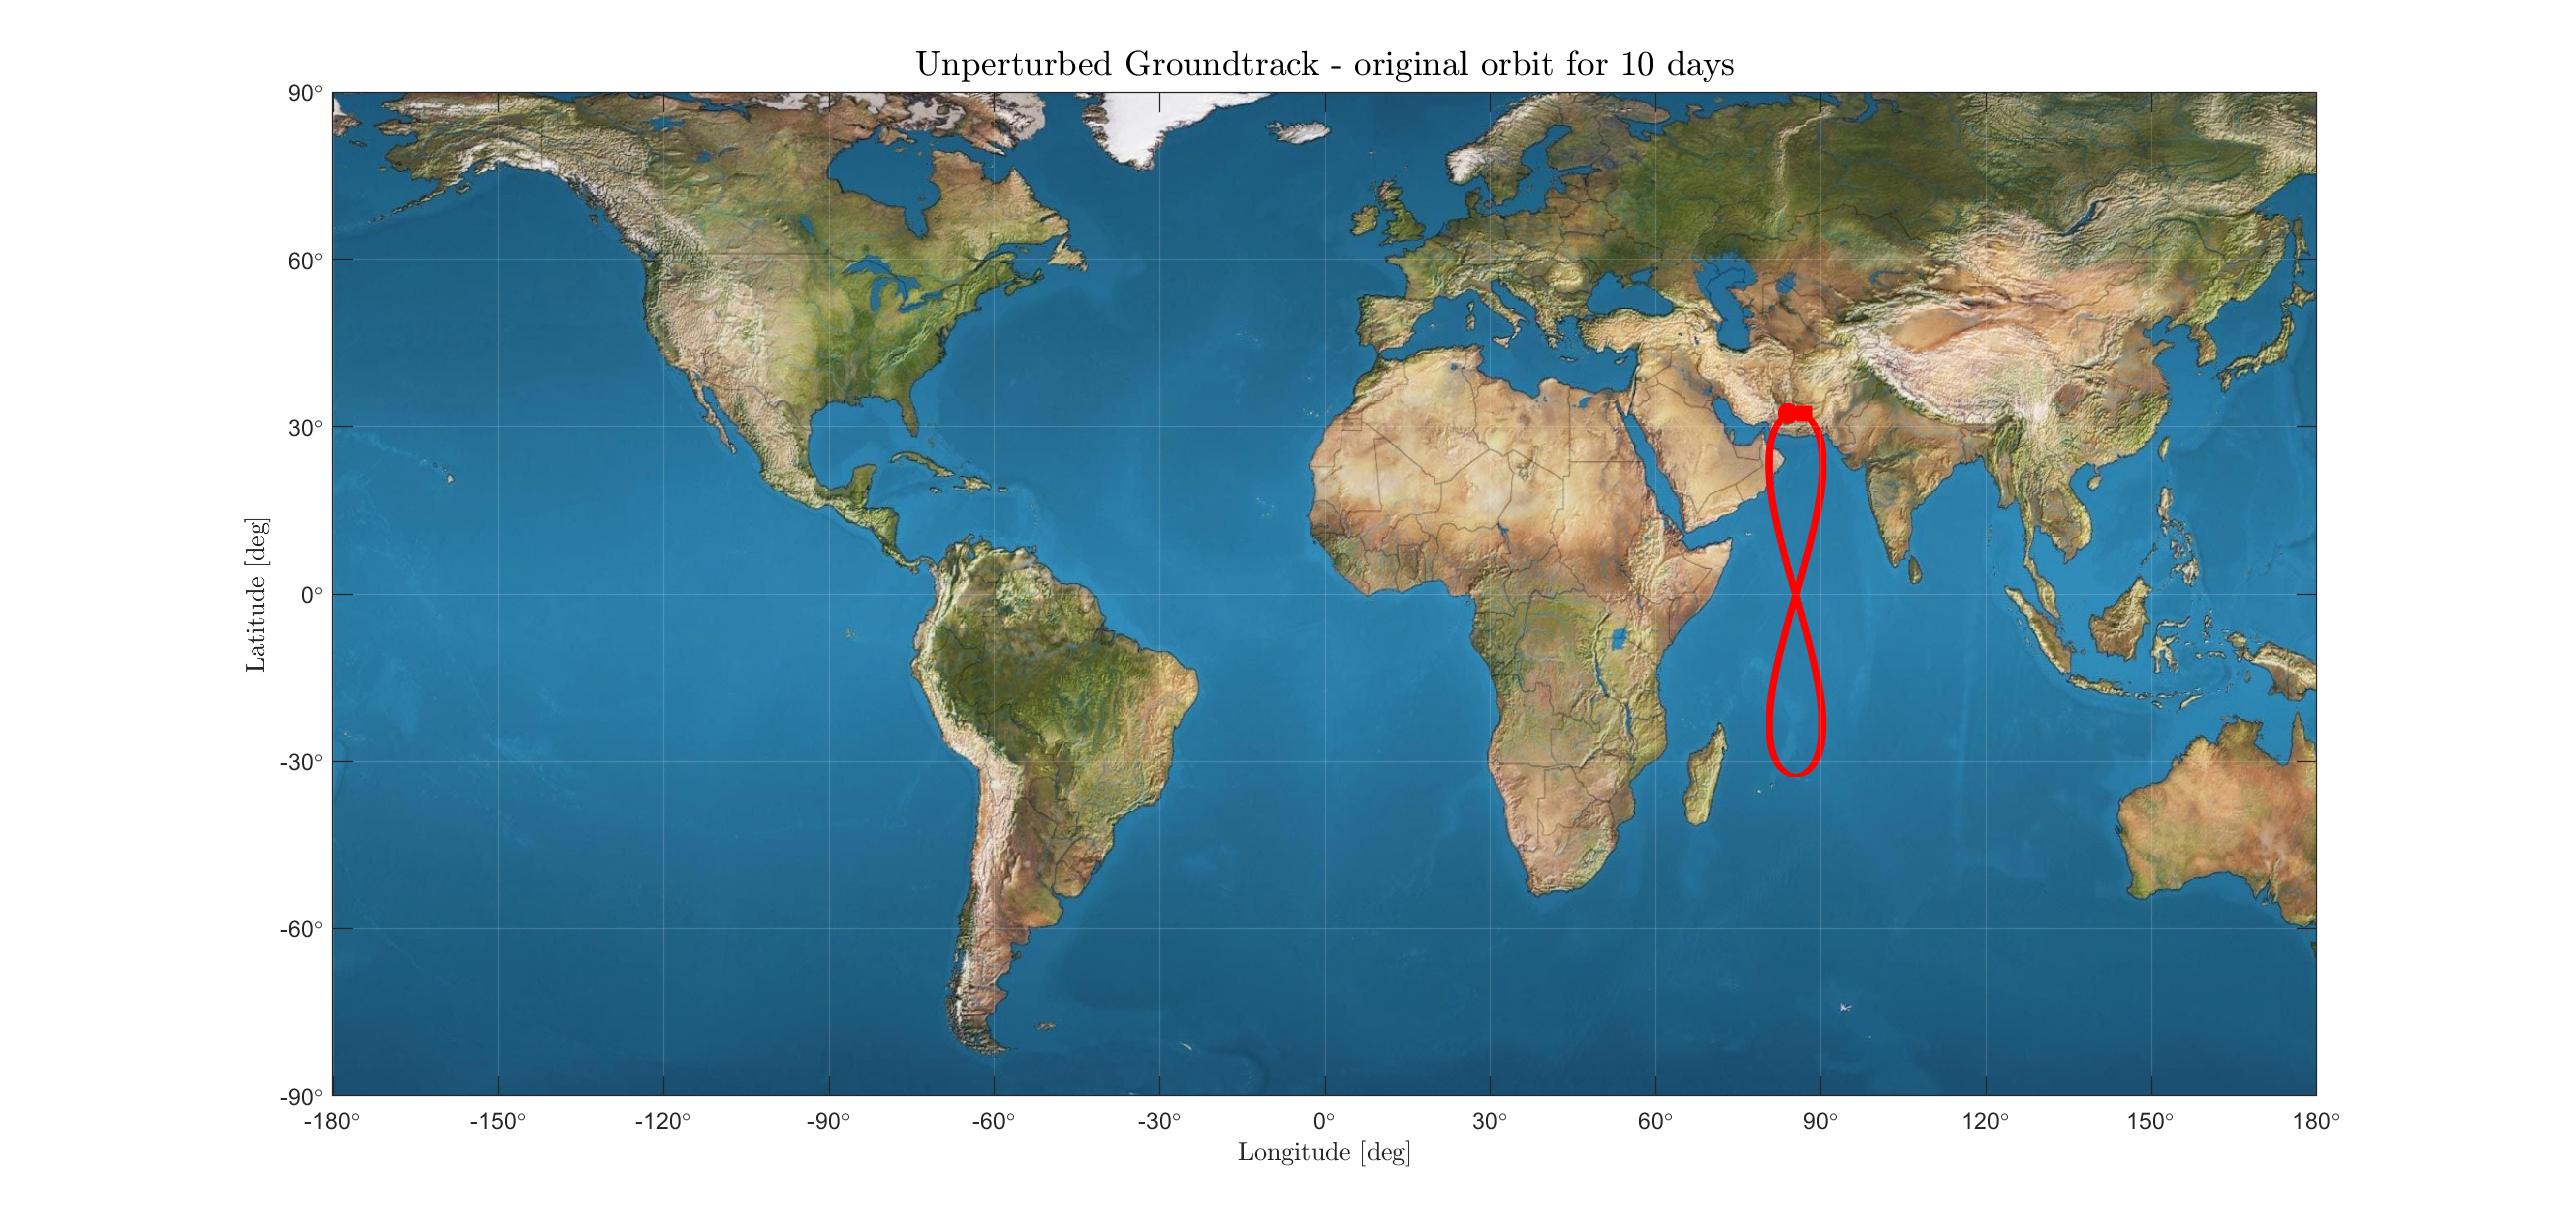
\includegraphics[width=\textwidth]{ug10d.png}
		\caption{}
		\label{fig:1c}
	\end{subfigure}
	\hfill
	\begin{subfigure}[b]{0.45\textwidth}
		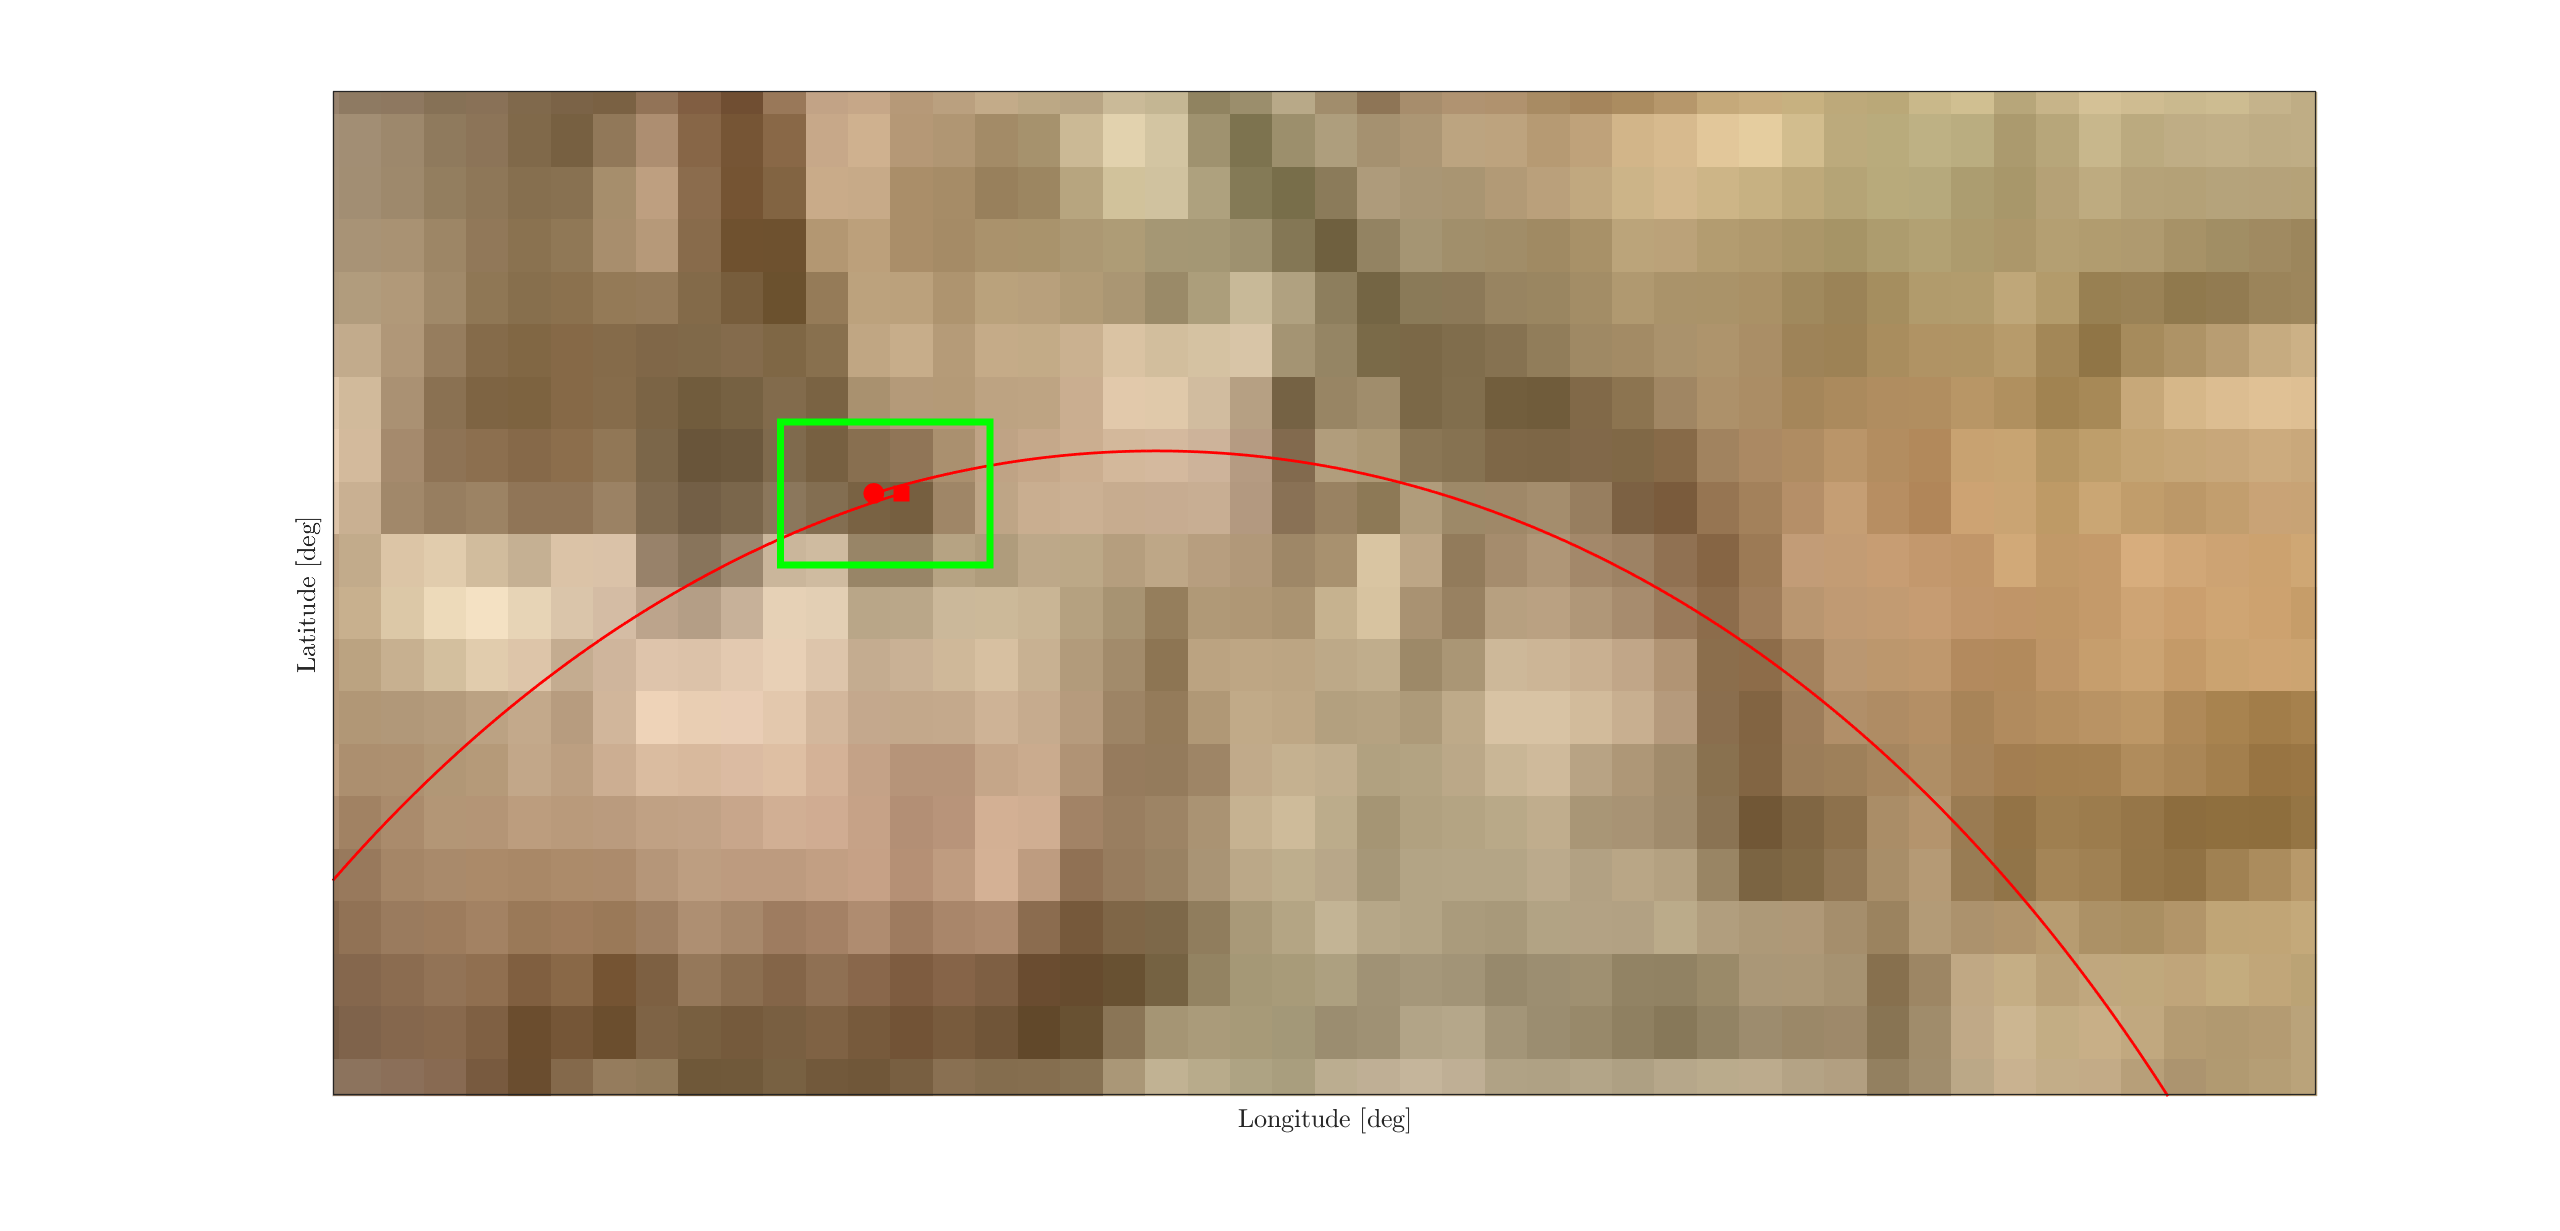
\includegraphics[width=\textwidth]{ugstartend.png}
		\caption{}
		\label{fig:1d}
	\end{subfigure}
	\caption{Ground track of the unperturbed nominal orbit during: (a) 1 orbit; (b) 1 day; (c) 10 days. Ground track path (\reddashedline), Starting point (\textcolor{red}{$\bullet$}), Ending point (\textcolor{red}{$\blacksquare$})
	}
\end{figure}

\begin{flushleft}
	The groundtrack of this satellite has formed an "8" shape, a phenomenon known as the figure-eight groundtrack. At geosynchronous altitude, the location after one revolution is the same, and for geostationary  orbits, the satellite always appears to be stationary over one location. The figure “8” occurs because the satellites relative velocity is less and greater, than locations on the Earth as it travels from the ascending node. 
\end{flushleft}

%cite: Vallado, Fundamentals of Astrodynamics, 2013

\subsubsection{Repeating Groundtrack}


For establishing a good communication with the network of ground stations of PoliMi Space Agency, a repeating ground track with a ratio of 1:1 (for each orbit of the spacecraft, Earth has performed 1 revolution) is maintained. Therefore, the period of the repeating ground track orbit is computed. For an unperturbed orbit, the period is only a function of the semi-major axis and can be calculated to get the desired repeating ground track. Both equations are listed as below. By extension, the other orbital parameters are kept the same as nominal orbit. 

	
\begin{equation*}
	T_{\text{repeating}} = \frac{1}{1} T_{\text{Earth}}
\end{equation*}

\begin{equation*}
	T = 2\pi \sqrt{\frac{a^3}{\mu}} \rightarrow a_{\text{repeating}} = \SI{42166}{\kilo\meter}
\end{equation*} 

\begin{figure}[ht]
	\centering
	\begin{subfigure}[b]{0.45\textwidth}
		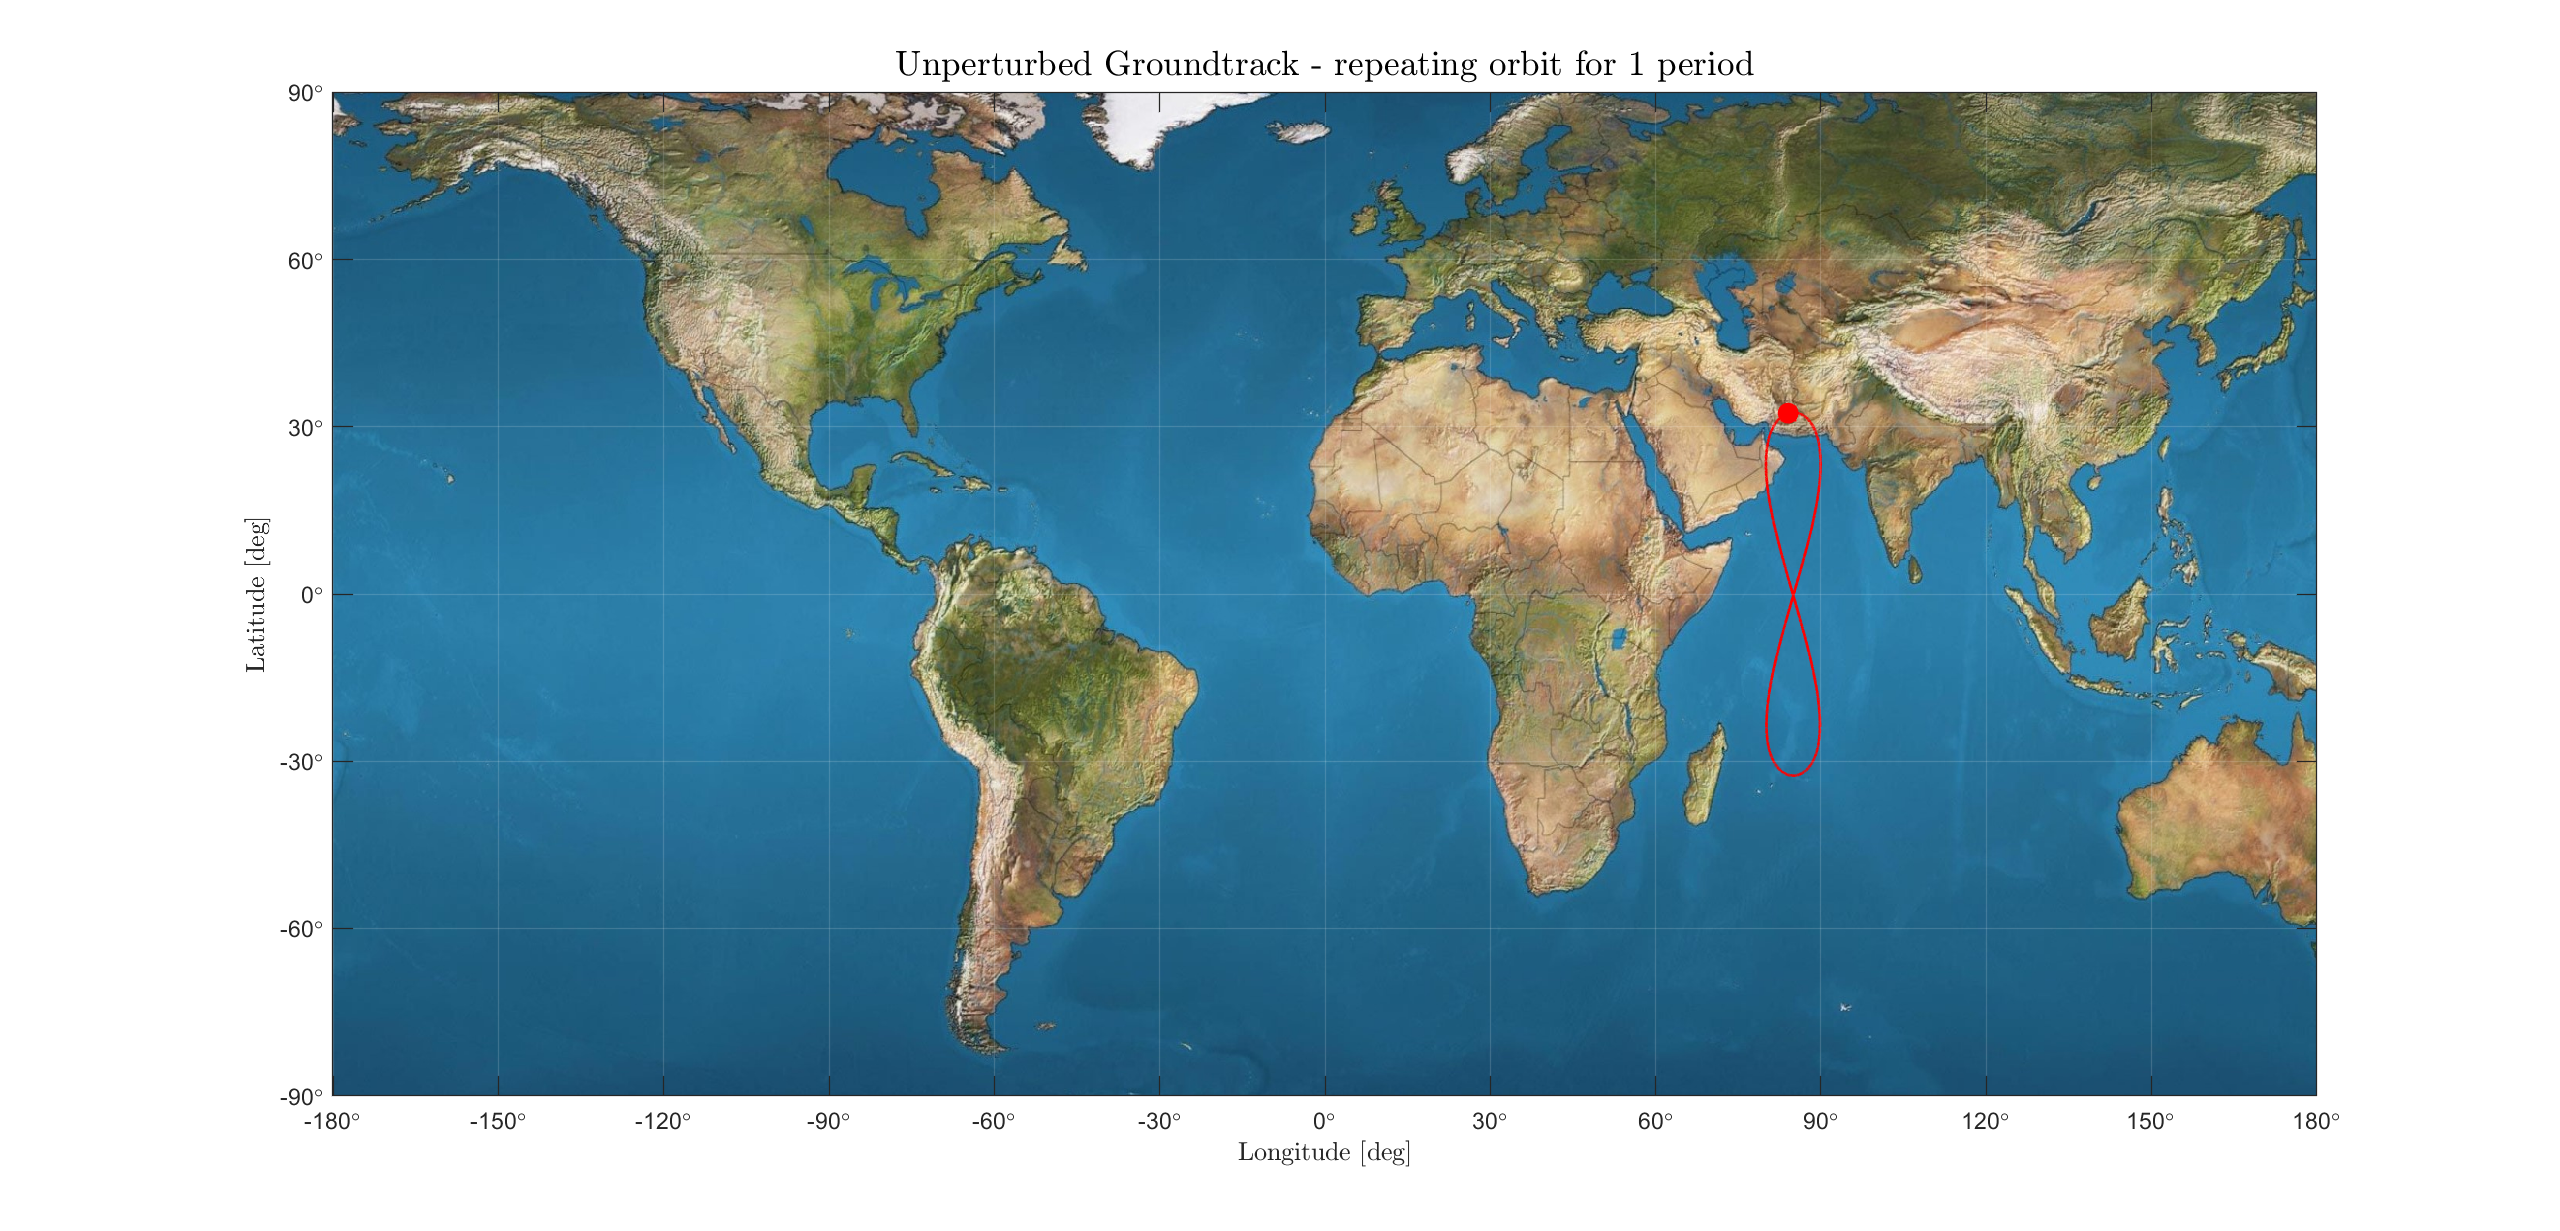
\includegraphics[width=\textwidth]{ugro1orb.png}
		\caption{}
		\label{fig:1a}
	\end{subfigure}
	\hfill
	\begin{subfigure}[b]{0.45\textwidth}
		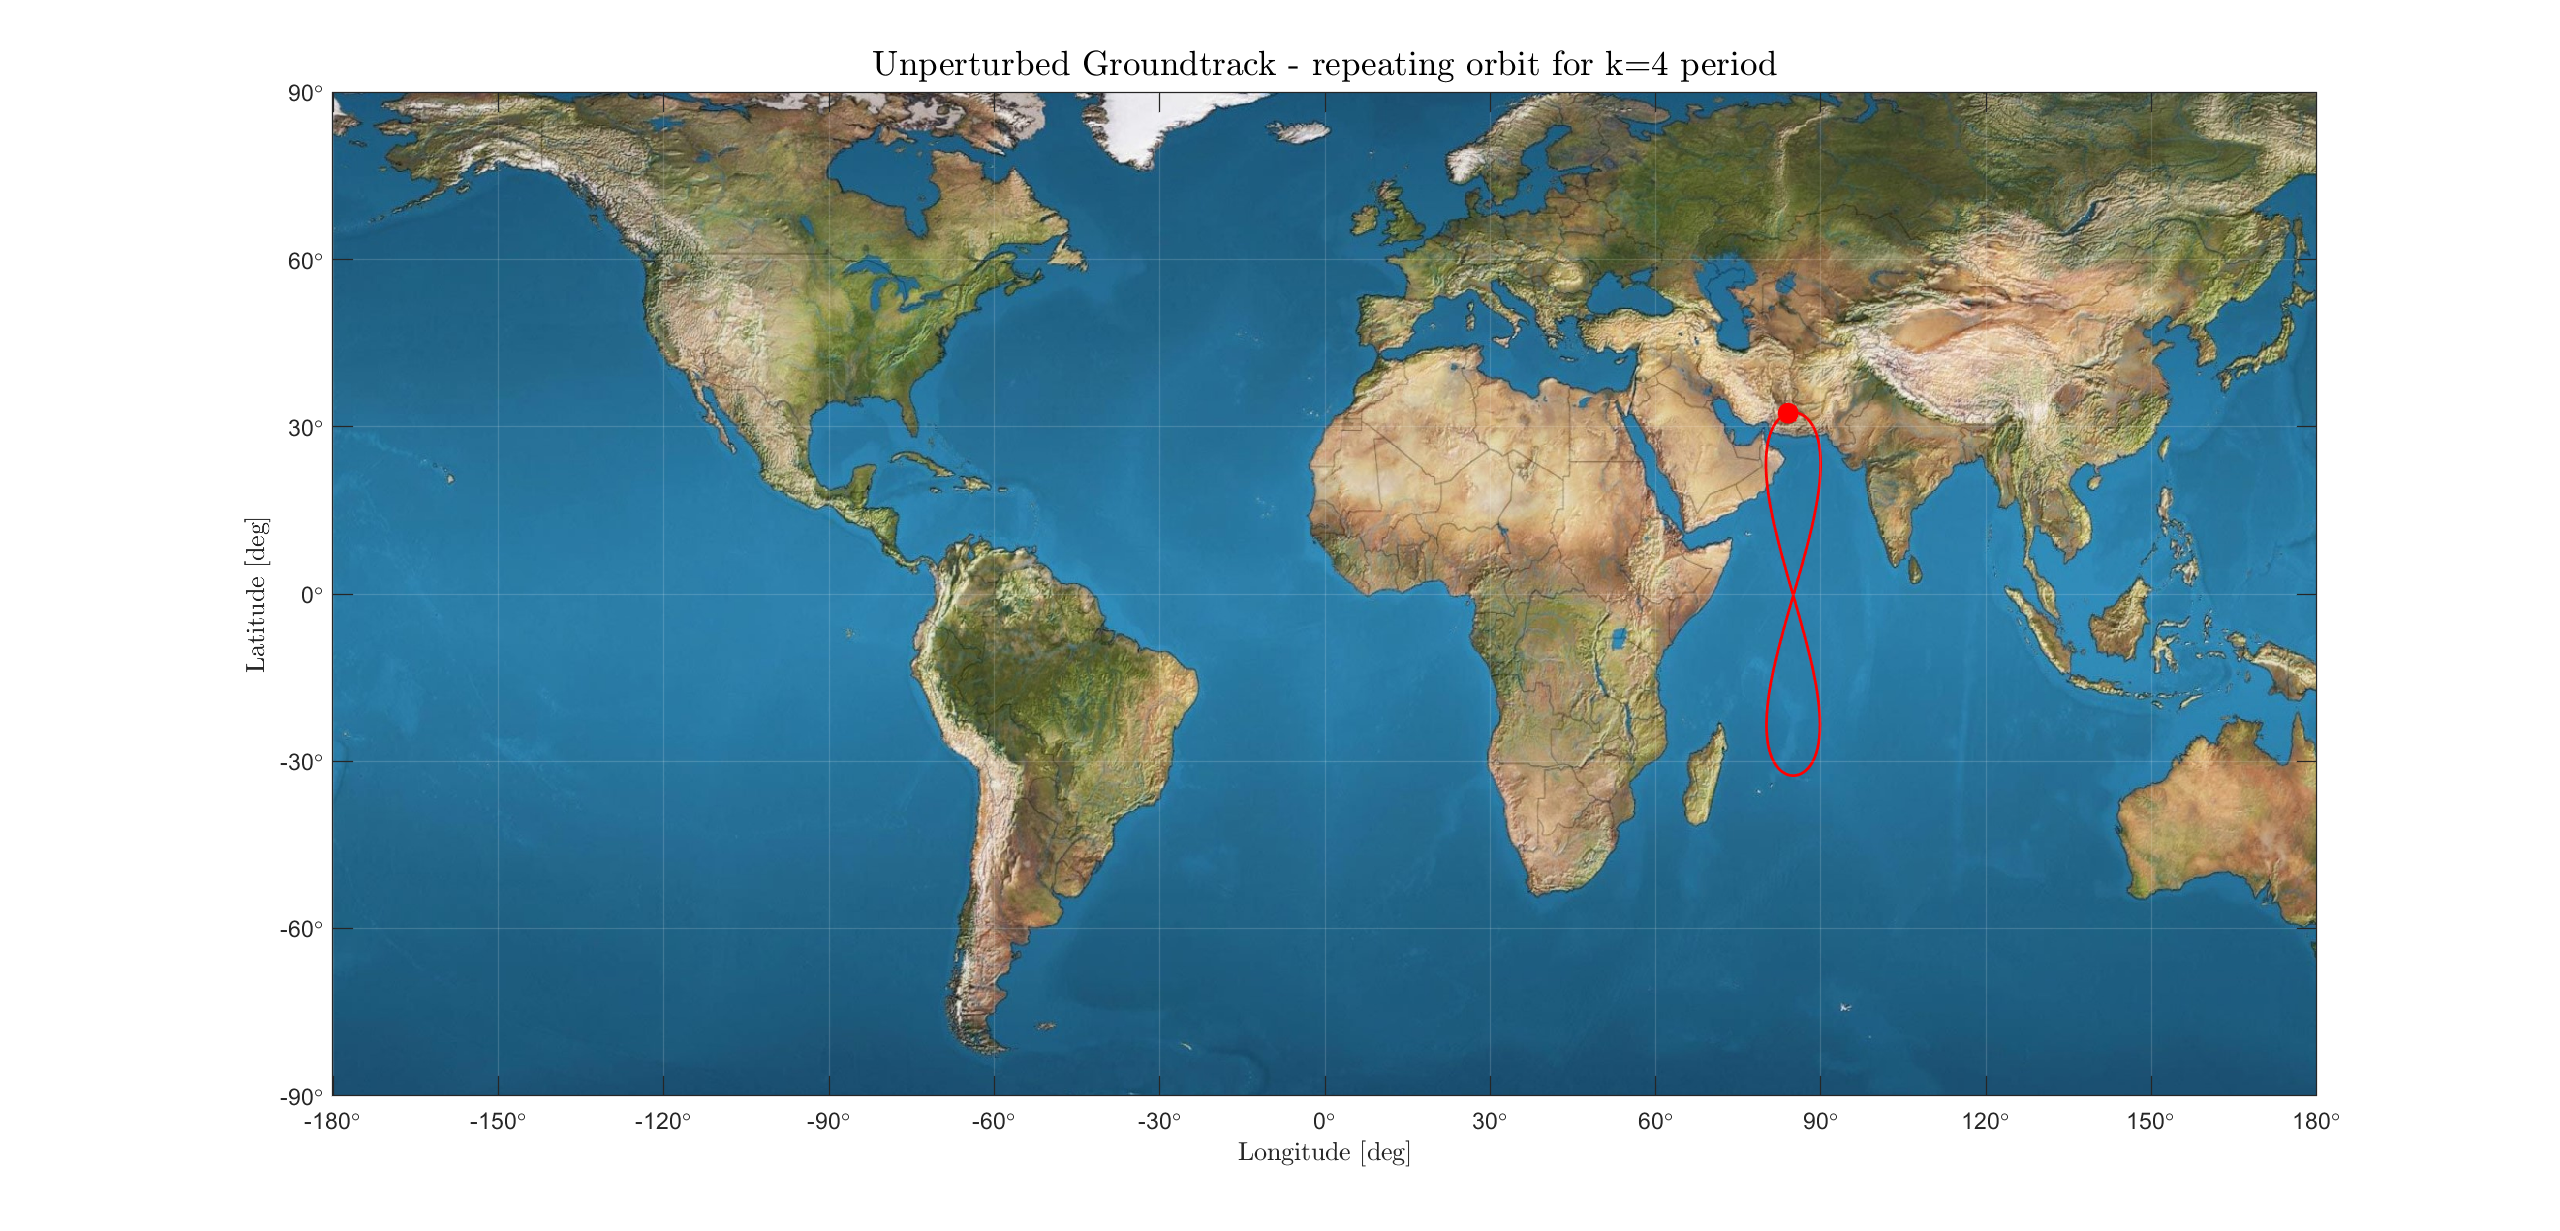
\includegraphics[width=\textwidth]{ugro4orb.png}
		\caption{}
		\label{fig:1b}
	\end{subfigure}
	
	\caption{Ground track of the unperturbed repeating orbit during: (a) 1 orbit; (b) 4·k=4 orbits. Ground track path (\reddashedline), Starting point (\textcolor{red}{$\bullet$}), Ending point (\textcolor{red}{$\blacksquare$})
	}
\end{figure}

\subsection{Perturbed Groundtrack}

	






	

	
\end{document}
